% LTeX: enabled=false
\documentclass[a4paper,11pt,oneside]{article}

\usepackage{placeins}

\makeatletter
\AtBeginDocument{%
  % Modifying section command to include FloatBarrier
  \expandafter\renewcommand\expandafter\section\expandafter
    {\expandafter\@fb@secFB\section}%
  % Modifying subsection command to include FloatBarrier
  \expandafter\renewcommand\expandafter\subsection\expandafter
    {\expandafter\@fb@secFB\subsection}%
  
  \newcommand\@fb@secFB{\FloatBarrier
    \gdef\@fb@afterHHook{\@fb@topbarrier \gdef\@fb@afterHHook{}}}%
  
  \g@addto@macro\@afterheading{\@fb@afterHHook}%
  \gdef\@fb@afterHHook{}%
}
\makeatother

\usepackage[english]{babel}

\usepackage[T1]{fontenc}

\usepackage[utf8]{inputenc}

\usepackage{graphicx}
\usepackage{cite}
\usepackage{url}
\usepackage{ifthen}
\usepackage{listings}
\usepackage{xcolor}
\usepackage{blindtext} % https://tex.stackexchange.com/questions/111948/what-is-a-overfull-hbox-9-89561pt-too-wide

\usepackage{helvet} % Add sans-serif font package
\renewcommand{\familydefault}{\sfdefault} % Set sans-serif as default

\graphicspath{{images/}}

\usepackage[hidelinks]{hyperref}
\usepackage{url}



\def \lstlistingname {SQL}
\lstset{
  language=SQL,
  tabsize=2,
  numbers=left,
  frame=L,
  floatplacement=hbtp,
  basicstyle=\ttfamily\small,
  keywordstyle=\color{blue},
  stringstyle=\color{red},
  commentstyle=\color{gray},
  captionpos=b, % This sets the caption below the listing
  showstringspaces=false,
  literate={'}{{\textquotesingle}}1
}

% LTeX: enabled=true

\title{Database Methodology - SQLite Implementation Tools}

% Write the name and user namn for all contributors, se below for \and
\author{Edwin Sundberg \url{edwin.sundberg@dsv.su.se} \and Melle Carnesten \url{melle.carnesten@dsv.su.se}}
% \and Person 2 \url{username2}

\begin{document}

\maketitle \pagebreak

% https://tex.stackexchange.com/questions/111948/what-is-a-overfull-hbox-9-89561pt-too-wide
\begin{sloppypar}  

\tableofcontents \pagebreak

% No one to thank yet
% \section{Acknowledgements}
% \label{acknowledgements}
% Thank you to the following people for reporting issues and contributing to this document:
% \begin{itemize}
%     \item Person 1 \url{username1}
%     \item Person 2 \url{username2}
%     \item Person 3 \url{username3}
% \end{itemize}

% TODO: Don't write "we", "I" or "us".

% TODO: Consistently use DBeaver Community or DBeaver, not both. (prob should be done with definition)

\section{The Database Model}
\label{exampleDatabaseModel}
In this document we will be using a simple database model which represents an email system, where users are able to create multiple recipient addresses and receive all incoming emails to one or more inboxes. All inboxes can be shared with other users in the system and receiving email may optionally be encrypted with a provided public key (see \url{https://en.wikipedia.org/wiki/Public-key_cryptography}). 
% TODO: Use cite for url instead

The original domain correct UML class diagram can be seen in figure \autoref{fig:originalUMLClassDiagram}. And the corresponding database model can be seen in figure \autoref{fig:originalDatabaseModel}. This document will not go into details on how or why the database model is created this way but rather focus on how to use the SQLite Modelling Tools to implement the database model. For details on how to go to a RDBMS friendly model from a domain model see lecture slides and literature.

% model/{database_friendly, instance, original_uml_class_diagram}.png
\begin{figure}[htb]
    \centering
    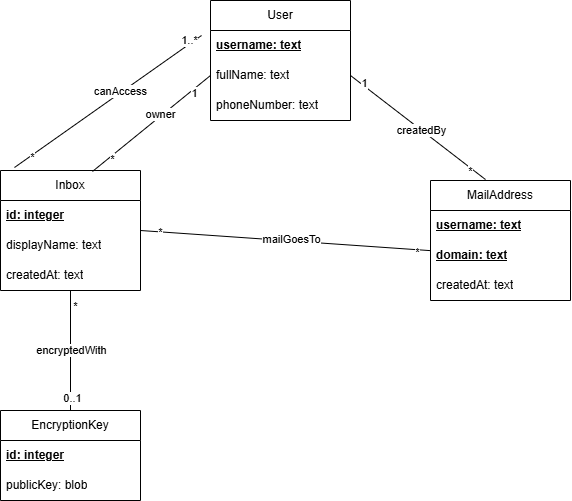
\includegraphics[width=1\textwidth]{model/original_uml_class_diagram.png}
    \caption{The original UML class diagram for the email system.}
    \label{fig:originalUMLClassDiagram}
\end{figure}

\begin{figure}[htb]
    \centering
    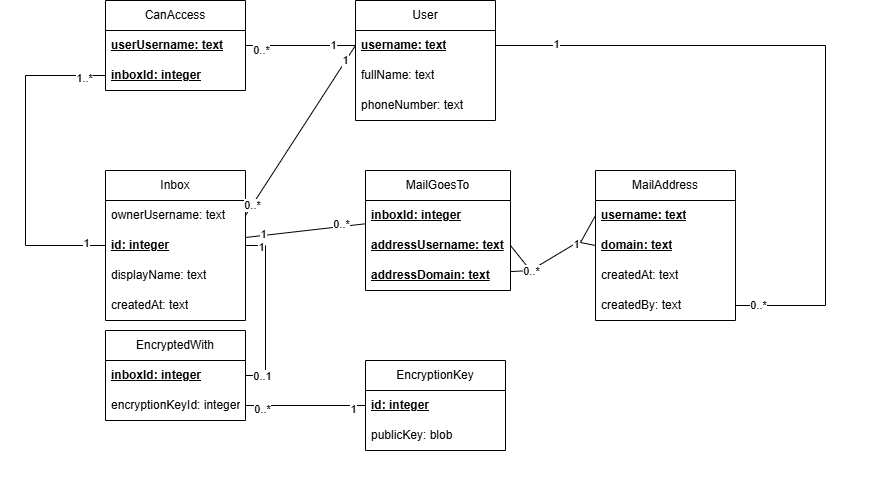
\includegraphics[width=1\textwidth]{model/database_friendly.png}
    \caption{The database model for the email system.}
    \label{fig:originalDatabaseModel}
\end{figure}

To further exemplify the database model we will also provide an instance of the database model in figure \autoref{fig:instanceDatabaseModel}. This instance will be used in the examples below to show how to insert data using the SQLite Implementation Tools.

\begin{figure}[htb]
    \centering
    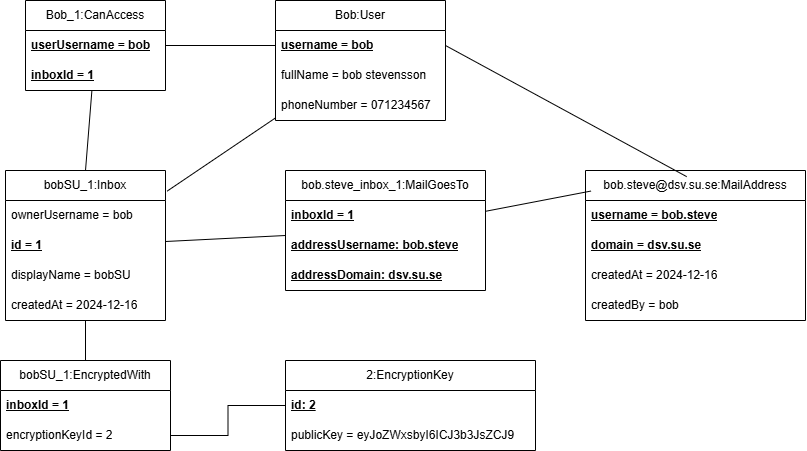
\includegraphics[width=1\textwidth]{model/instance.png}
    \caption{An instance of the database model for the email system.}
    \label{fig:instanceDatabaseModel}
\end{figure}

\section{The SQLite Implementation Tools}
\label{sqliteImplementationTools}
The following tools will be presented in this document:
\begin{itemize}
    \item DBeaver Community (see \autoref{dbeaverCommunity})
    \item SQLiteStudio (see \autoref{sqliteStudio})
    \item SQLite ERD (see \autoref{sqliteERD})
\end{itemize}
along with some specifics of SQLite in general (see \autoref{sqliteInGeneral}).

\section{SQLite in General}
\label{sqliteInGeneral}

\subsection{Datatypes}
\label{sqliteDatatypes}
Typing is not strict in SQLite, but we recommend to stick to the following datatypes for the database model:
\begin{itemize}
  \item INTEGER
  \item TEXT
  \item REAL
  \item BLOB (Binary Large Object)
\end{itemize}
While typing is not strict it is still highly recommended to insert data of the correct type to avoid logical errors, i.e. only insert integers into INTEGER columns and no strings into INTEGER columns. Note: SQLite ERD (see \autoref{sqliteERD}) will throw semantic errors if there exists data of the ``wrong'' type in a column.

\subsection{Date and Time Management}
\label{sqliteDateTime}

Since there does not exist a specific datatype for date and time in SQLite, the official recommendation is to store it in one of the following formats: \cite{sqlite_date_time}
\begin{itemize}
  \item TEXT - containing ISO-8601 strings (e.g. ``YYYY-MM-DD HH:MM:SS.SSS'' or ``YYYY-MM-DD'')
  \item INTEGER - Unix Time (see \url{https://www.unixtimestamp.com/})
  \item REAL - Julian Day Number (see \url{https://en.wikipedia.org/wiki/Julian_day})
\end{itemize}

\subsubsection{Handling Dates Correctly}
There are a few approaches to handle dates correctly in SQLite, the following are some examples of querying all ``inboxes'' that have been created during the year 2025:

\begin{lstlisting}[caption={Querying using BETWEEN}, label={lst:sqliteBetween}]
SELECT
  *
FROM
  inboxes
WHERE
  createdAt BETWEEN '2025-01-01' AND '2025-12-31';
\end{lstlisting}

\begin{lstlisting}[caption={Querying using strftime}, label={lst:sqliteStrftime}]
SELECT
    *
FROM
    inboxes
WHERE
    -- The strftime function extracts the year (%Y) from
    -- the 'createdAt' column.
    -- It returns the year as a text
    -- string (e.g., '2025').
    CAST(
        strftime('%Y', createdAt)
        AS INT  -- The CAST converts the year string to 
                -- an integer for numeric comparison.
    ) = 2025;
\end{lstlisting}

For a complete list of possible parameters to ``strftime'' used in \autoref{lst:sqliteStrftime} see \cite{sqlite_date_time}.

The solutions presented above will work independently of the format the date is stored in the database (i.e. TEXT, INTEGER, REAL) assuming the datatype matches the format as explained in \autoref{sqliteDateTime}.

\subsubsection{Anti-examples of Date and Time Management}

The following are anti-examples of how to \textbf{not} handle dates in SQLite. The following examples may produce unexpected results and should be avoided as they handle the date as a string and not as a date and will completely break if Unix Time or Julian Day Number is used (or switched to) as the storage format.

\begin{lstlisting}[caption={Anti-example of date querying using LIKE}, label={lst:sqliteLike}]
SELECT
  *
FROM
  inboxes
WHERE
  -- Matches all strings starting with
  -- '2025' (e.g. '2025HELLO').
  createdAt LIKE '2025%';
\end{lstlisting}

\begin{lstlisting}[caption={Anti-example of date querying using >=}, label={lst:sqliteGreaterEqual}]
SELECT
  *
FROM
  inboxes
WHERE
  -- Matches all strings starting with
  -- '2025' (e.g. '2025HELLO').
  createdAt >= '2025';
OR
  -- Is internally casted to the same as above.
  createdAt >= 2025;
\end{lstlisting}

\begin{lstlisting}[caption={Anti-example of date querying with incorrect BETWEEN}, label={lst:sqliteBetweenIncorrect}]
SELECT
  *
FROM
  inboxes
WHERE
  -- This will return an undefined result set since
  -- DD/MM/YYYY is not ISO-8601 format.
  createdAt BETWEEN '01/01/2025' AND '12/31/2025';
\end{lstlisting}



\section{DBeaver Community}
\label{dbeaverCommunity}

\subsection{Relevant Known Issues}
\label{dbeaverKnownIssues}

\subsubsection{Bad Primary Key due to auto increment}
When creating an integer column in DBeaver Community with the ``auto increment'' box checked the SQL generated will have a PK constraint created twice. This will result in an error when trying to persist the changes since a table can only have one PRIMARY KEY constraint. The following code is generated by DBeaver Community when trying to persist the changes:
\begin{lstlisting}[caption={Bad Primary Key due to auto increment in DBeaver}]
CREATE TABLE BadPK (
	Column1 INTEGER NOT NULL PRIMARY KEY AUTOINCREMENT,
	CONSTRAINT BadPK_PK PRIMARY KEY (Column1)
);
\end{lstlisting}
The solution to this is to never use the ``auto increment box'' (for a SQLite database in DBeaver) when creating a PK in the program. Unchecking the box will instead yield the following code:
\begin{lstlisting}[caption={Ok Primary Key in DBeaver if auto increment is unchecked}]
CREATE TABLE GoodPK (
	Column1 INTEGER NOT NULL,
	CONSTRAINT GoodPK_PK PRIMARY KEY (Column1)
);
\end{lstlisting}
For more information on why this is the case see \cite{dbeaver_issue_18491}.


\subsection{Common Problems}
\label{dbeaverCommonProblems}

\subsubsection{Foreign Key Constraints are not enforced}
\label{dbeaverForeignKeysNotEnforced}
DBeaver does not enforce foreign key constraints by default. This can either be enabled when creating a new database (see \autoref{dbeaverCreatingDatabase}) or by editing the database connection settings as follows:
\begin{enumerate}
    \item Right-click on the connection and choose ``Edit Connection''. (\autoref{fig:edit_connection})
    \item Go to ``Connection settings'' → ``Driver properties'' (\autoref{fig:edit_driver_properties}).
    \item Locate and change ``Foreign keys'' to ``true'' (\autoref{fig:edit_foreign_keys_enable}).
    \item Press ``OK'' and reconnect if necessary.
\end{enumerate}

\begin{figure}[!htb]
  \centering
  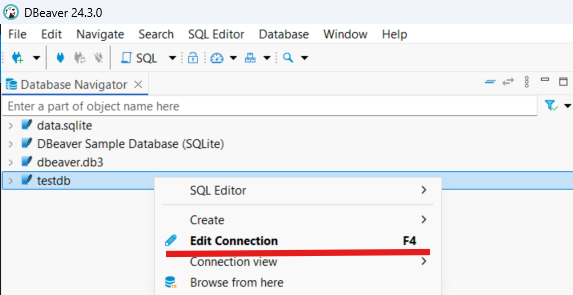
\includegraphics[width=0.7\textwidth]{dbeaver/edit_connection.png}
  \caption{Edit Connection in DBeaver.}
  \label{fig:edit_connection}
\end{figure}

\begin{figure}[!htb]
  \centering
  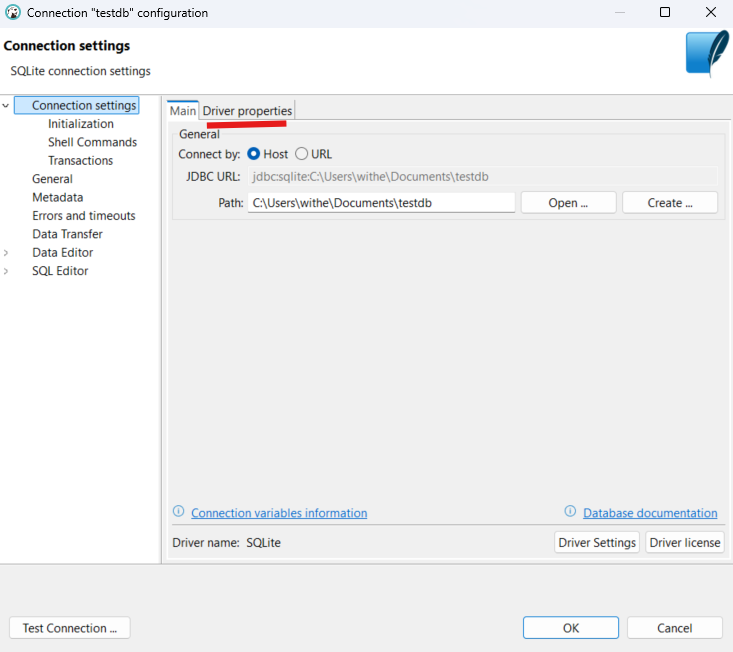
\includegraphics[width=0.7\textwidth]{dbeaver/edit_driver_properties.png}
  \caption{Driver Properties in DBeaver.}
  \label{fig:edit_driver_properties}
\end{figure}

\begin{figure}[!htb]
  \centering
  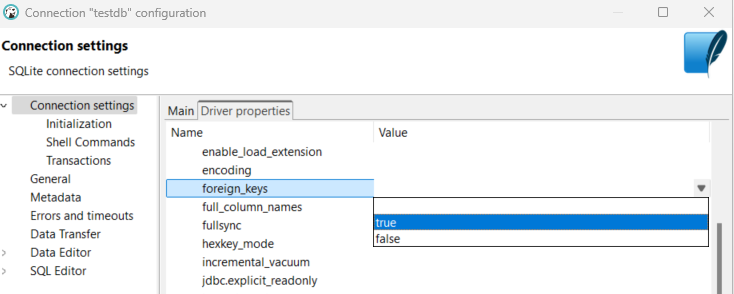
\includegraphics[width=0.7\textwidth]{dbeaver/edit_foreign_keys_enable.png}
  \caption{Enable Foreign Keys in DBeaver.}
  \label{fig:edit_foreign_keys_enable}
\end{figure}

\subsubsection{ERD Created Foreign Key Constraints}
\label{dbeaverERDCreatedForeignKeys}
The ERD tool in DBeaver Community allows you to drag tables/columns to create ``virtual keys'' which are not saved in the database itself - per the DBeaver documentation:
``Note: Virtual keys exist only in DBeaver, not in the database itself. You can define these keys even if your database does not support them''. \cite{dbeaver_virtual_keys} So do not rely on the ERD tool to create foreign key constraints in the database itself, instead follow the steps outlined in \autoref{dbeaverForeignKeys}.

\subsubsection{Editing a Column}
\label{dbeaverEditingColumn}
It is not possible to change a column's datatype/NULL constraint/etc. after creation in DBeaver Community. The only way to change a column is to create a new column with the desired properties, copy the data (if applicable) over and subsequently delete the old column.

% \subsection{Implementation of the Database Model}
% \label{dbeaverImplementation}

\subsection{Creating Databases}
\label{dbeaverCreatingDatabase}
To create a new database with foreign key constraints enabled in DBeaver Community:
\begin{enumerate}
    \item Press ``New Database Connection'' (\autoref{fig:new_database_connection}).
    \item Choose SQLite, press ``Next''. (\autoref{fig:new_database_sqlite})
    \item Choose a file location for the database with ``Create...'' ensure to name the file with the extension ``.db3'' or ``.sqlite3'' (\autoref{fig:create_choose_file_location}).
    \item Go to ``Driver Properties'' and change ``Foreign keys'' to ``true'' (\autoref{fig:create_foreign_keys_enable}).
    \item Press ``Finish''.
\end{enumerate}

\begin{figure}[!htb]
  \centering
  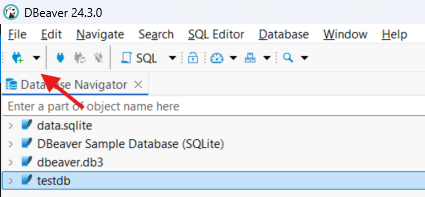
\includegraphics[width=0.7\textwidth]{dbeaver/new_database_connection.png}
  \caption{New Database Connection in DBeaver.}
  \label{fig:new_database_connection}
\end{figure}

\begin{figure}[!htb]
  \centering
  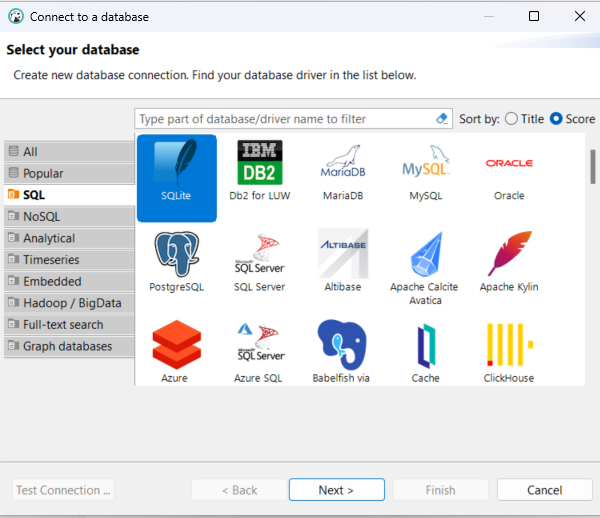
\includegraphics[width=0.7\textwidth]{dbeaver/new_database_sqlite.png}
  \caption{New SQLite Database in DBeaver.}
  \label{fig:new_database_sqlite}
\end{figure}

\begin{figure}[!htb]
  \centering
  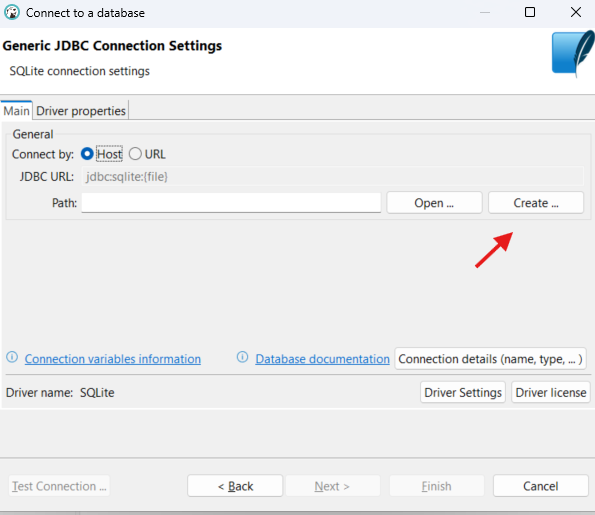
\includegraphics[width=0.7\textwidth]{dbeaver/create_choose_file_location.png}
  \caption{Choose File Location in DBeaver.}
  \label{fig:create_choose_file_location}
\end{figure}

\begin{figure}[!htb]
  \centering
  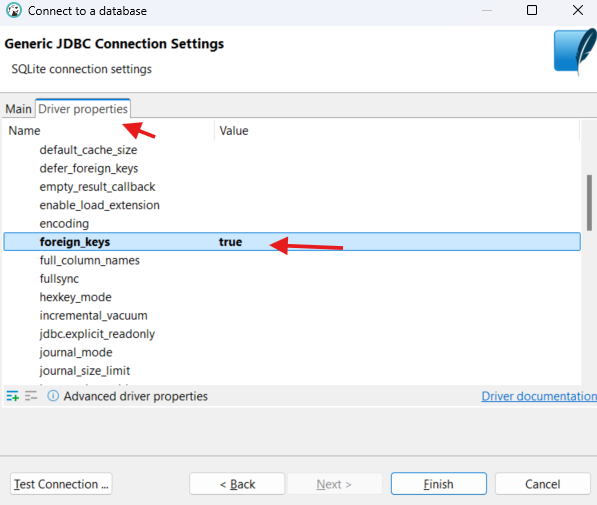
\includegraphics[width=0.7\textwidth]{dbeaver/create_foreign_keys_enable.png}
  \caption{Enable Foreign Keys in DBeaver.}
  \label{fig:create_foreign_keys_enable}
\end{figure}



\subsection{Creating Tables}
\label{dbeaverCreatingTable}
% TODO: and breifly mention MailGoesTo table
From the database model, we will be implementing the User and the MailAddress tables. The rest of the tables can be implemented similarly and is left as an exercise for the reader.

\subsubsection{User Table}
\label{dbeaverUserTable}

\begin{enumerate}
  \item \label{dbeaverCreateTable} Expand the database connection and right-click on ``Tables'' and choose ``Create New Table'' (\autoref{fig:create_new_table}).
  \item Fill out the Table Name field, navigate to the ``Columns'' tab, right click and choose ``Add Column'' (\autoref{fig:name_and_add_column}).
  \item \label{dbeaverAddColumn} Add the column for username, set the datatype to ``TEXT'', check the box for ``NOT NULL'' and the box for ``Unique'' in order to create a single column primary key (\autoref{fig:username_primary_key}).
  \item Repeat step \ref{dbeaverAddColumn} for the columns ``fullName'' and ``phoneNumber'' but without checking the box for ``Unique''.
  \item Save with ``Ctrl + S'' (or your operating system's equivalent) and press ``Execute''.
  \item The resulting table can be visualized using DBeaver's built in ER Diagram tool (\autoref{fig:user_er_diagram}). 
\end{enumerate}

\begin{figure}[!htb]
  \centering
  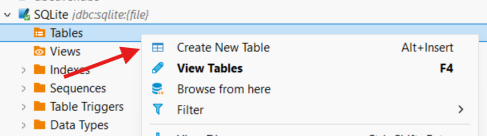
\includegraphics[width=0.7\textwidth]{dbeaver/create_new_table.png}
  \caption{Create New Table in DBeaver.}
  \label{fig:create_new_table}
\end{figure}

\begin{figure}[!htb]
  \centering
  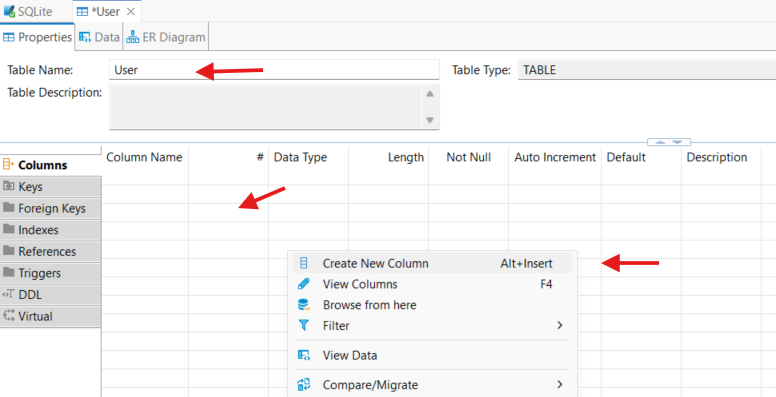
\includegraphics[width=0.7\textwidth]{dbeaver/name_and_add_column.png}
  \caption{Add Column in DBeaver.}
  \label{fig:name_and_add_column}
\end{figure}

\begin{figure}[!htb]
  \centering
  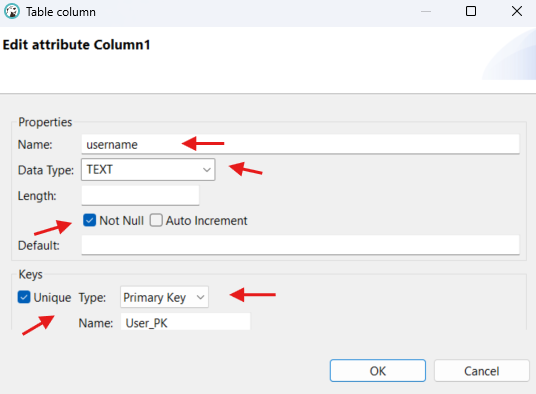
\includegraphics[width=0.7\textwidth]{dbeaver/username_primary_key.png}
  \caption{Username Primary Key in DBeaver.}
  \label{fig:username_primary_key}
\end{figure}

\begin{figure}[!htb]
  \centering
  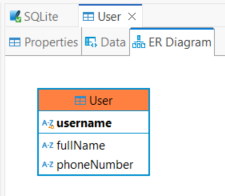
\includegraphics[width=0.7\textwidth]{dbeaver/user_er_diagram.png}
  \caption{User ER Diagram in DBeaver.}
  \label{fig:user_er_diagram}
\end{figure}


\subsubsection{MailAddress Table}
\label{dbeaverMailAddressTable}
The process for creating the MailAddress table is similar to the User table with the exception that the \textbf{primary key} is a composite key. The PK for the table consists of the columns ``username'' and ``domain''. Steps for creating columns are the same as for \ref{dbeaverUserTable}, creating the composite key is done as follows:
\begin{enumerate}
  \item Navigate to the ``Keys'' tab (\autoref{fig:table_keys_navigate}).
  \item Right click, choose ``Create New Key''
  \item Set the type to ``Primary Key'' and tick the columns ``username'' and ``domain'' to the key (\autoref{fig:mail_address_primary_key}).
  \item Press ``OK'' and save the table.
  \item The resulting table can be visualized using DBeaver's built in ER Diagram tool. (\autoref{fig:mail_address_er_diagram})
\end{enumerate}

\begin{figure}[!htb]
  \centering
  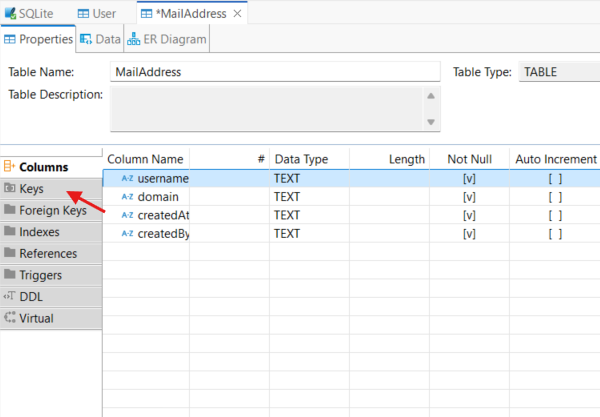
\includegraphics[width=0.7\textwidth]{dbeaver/table_keys_navigate.png}
  \caption{Navigate to Keys in DBeaver.}
  \label{fig:table_keys_navigate}
\end{figure}

\begin{figure}[!htb]
  \centering
  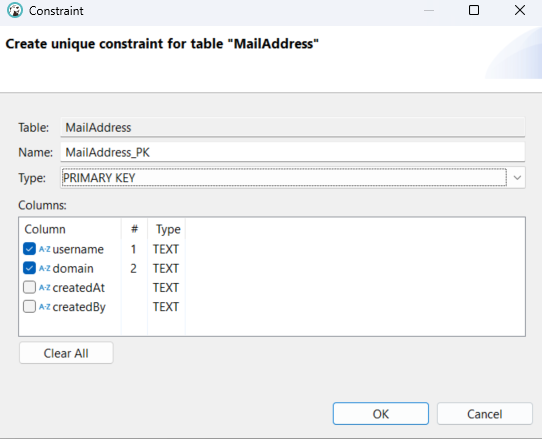
\includegraphics[width=0.7\textwidth]{dbeaver/mail_address_primary_key.png}
  \caption{MailAddress Primary Key in DBeaver.}
  \label{fig:mail_address_primary_key}
\end{figure}

\begin{figure}[!htb]
  \centering
  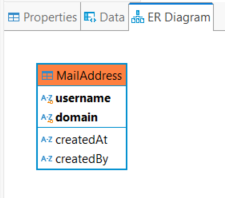
\includegraphics[width=0.7\textwidth]{dbeaver/mail_address_er_diagram.png}
  \caption{MailAddress ER Diagram in DBeaver.}
  \label{fig:mail_address_er_diagram}
\end{figure}

\subsubsection{MailGoesTo Table}
\label{dbeaverMailGoesToTable}
The process of creating the MailGoesTo table is almost identical to the \autoref{dbeaverMailAddressTable} with the exception that all columns are part of the primary key. The resulting table can be visualized with DBeaver as \autoref{fig:mail_goes_to_er_diagram}.

\begin{figure}[!htb]
  \centering
  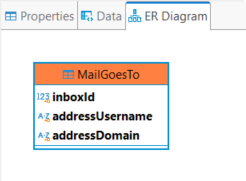
\includegraphics[width=0.7\textwidth]{dbeaver/mail_goes_to_er_diagram.png}
  \caption{MailGoesTo ER Diagram in DBeaver.}
  \label{fig:mail_goes_to_er_diagram}
\end{figure}

\subsection{Alternative Keys}
\label{dbeaverAlternativeKeys}
To create an alternative key (unique index) in DBeaver this can be exemplified on User by declaring that the columns ``fullName'' and ``phoneNumber'' should be unique together. This can be done as follows:

\begin{enumerate}
  \item Navigate to the ``Indexes'' tab in the User table (\autoref{fig:user_index_tab}).
  \item Right-click and choose ``Create New Index''.
  \item Select the columns ``fullName'' and ``phoneNumber'', tick the box for ``Unique'' and press ``OK''. (\autoref{fig:user_index_create})
\end{enumerate}

\begin{figure}[!htb]
  \centering
  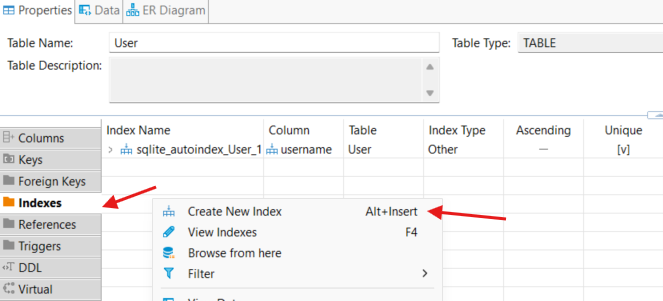
\includegraphics[width=0.7\textwidth]{dbeaver/user_index_tab.png}
  \caption{Navigate to Indexes in DBeaver.}
  \label{fig:user_index_tab}
\end{figure}

\begin{figure}[!htb]
  \centering
  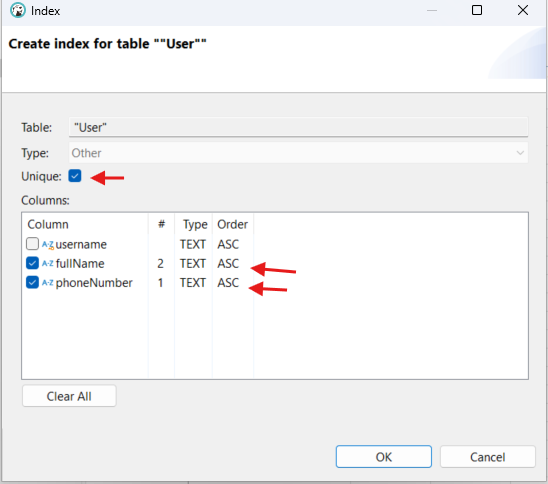
\includegraphics[width=0.7\textwidth]{dbeaver/user_index_create.png}
  \caption{Create Unique Index in DBeaver.}
  \label{fig:user_index_create}
\end{figure}


\subsection{Foreign Keys}
\label{dbeaverForeignKeys}
Creating foreign keys in DBeaver will be exemplified on the relationships between MailAddress.(createdBy) → User.(username) and MailGoesTo.(username, domain) → MailAddress.(username, domain).

\subsubsection{MailAddress → User}
\label{dbeaverUserMailAddressRelationship}
A single column foreign key relationship between User.(username) and MailAddress.(createdBy), can be created as follows:

\begin{enumerate}
  \item Navigate to the ``Foreign Keys'' tab of the MailAddress table.
  \item Right-click and choose ``Create New Foreign Key''. (\autoref{fig:navigate_create_foreign_key_tab}).
  \item Set the destination / ``reference'' table to User, the ``from'' column to createdBy and the reference column to username. (\autoref{fig:create_foreign_key_mail_address_user}).
  \item Set ``ON DELETE'' and ``ON UPDATE'' to appropriate values.
  \item Press ``OK'' and save the table.
\end{enumerate}

\begin{figure}[!htb]
  \centering
  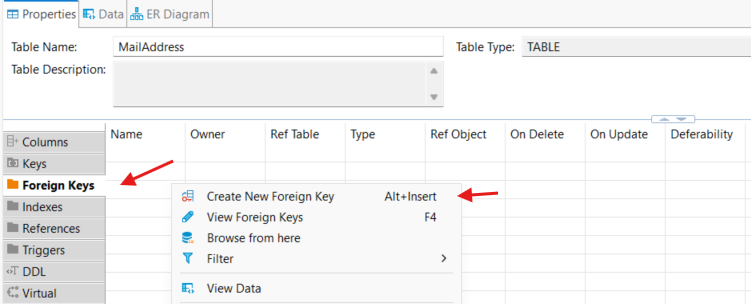
\includegraphics[width=0.7\textwidth]{dbeaver/navigate_create_foreign_key_tab.png}
  \caption{Navigate to Create Foreign Key in DBeaver.}
  \label{fig:navigate_create_foreign_key_tab}
\end{figure}

\begin{figure}[!htb]
  \centering
  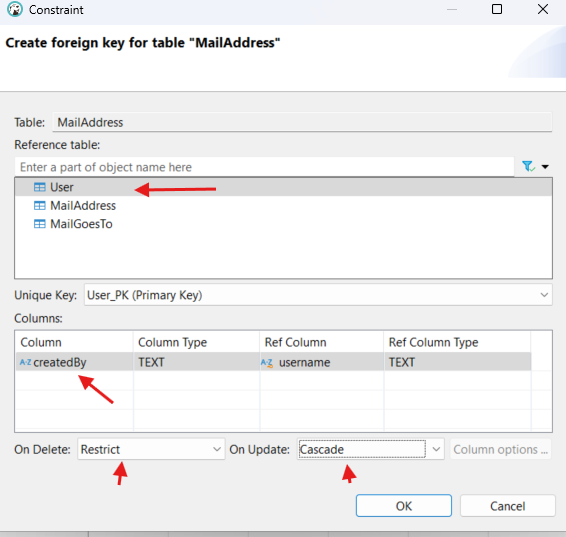
\includegraphics[width=0.7\textwidth]{dbeaver/create_foreign_key_mail_address_user.png}
  \caption{Create Foreign Key MailAddress → User in DBeaver.}
  \label{fig:create_foreign_key_mail_address_user}
\end{figure}



\subsubsection{MailGoesTo → MailAddress}
\label{dbeaverMailGoesToMailAddressRelationship}
A composite foreign key relationship between MailGoesTo.(addressUsername, addressDomain) and MailAddress.(username, domain), can be created as follows:

\begin{enumerate}
  \item Navigate to the ``Foreign Keys'' tab of the MailGoesTo table.
  \item Right-click and choose ``Create New Foreign Key''. (\autoref{fig:navigate_create_foreign_key_tab}).
  \item Set the destination / ``reference'' table to MailAddress, the ``from'' columns to username and domain and the reference columns to username and domain. (\autoref{fig:create_foreign_key_mail_goes_to_mail_address}).
  \item Set ``ON DELETE'' and ``ON UPDATE'' to appropriate values.
  \item Press ``OK'' and save the table.
\end{enumerate}

\begin{figure}[!htb]
  \centering
  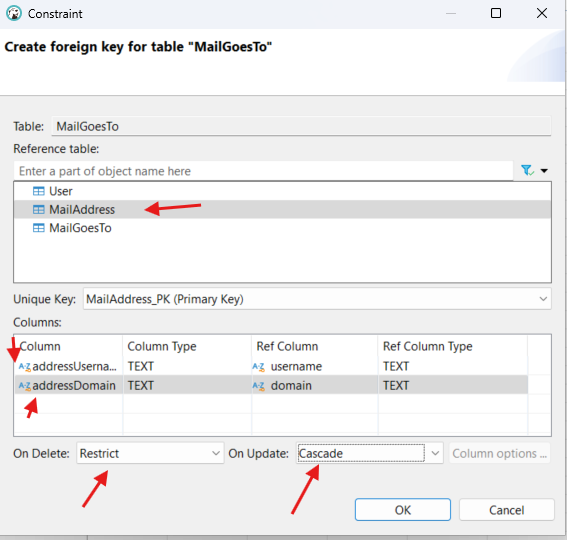
\includegraphics[width=0.7\textwidth]{dbeaver/create_foreign_key_mail_goes_to_mail_address.png}
  \caption{Create Foreign Key MailGoesTo → MailAddress in DBeaver.}
  \label{fig:create_foreign_key_mail_goes_to_mail_address}
\end{figure}


\subsection{Inserting Data}
\label{dbeaverInsertingData}

We will now insert data into the User and MailAddress tables. The data to be inserted can be seen in \autoref{fig:instanceDatabaseModel}. The process for inserting data is the same for all tables and can be exemplified on the User table as follows:

\begin{enumerate}
  \item Navigate to the ``Data'' tab of the User table.
  \item Right-click, choose ``Edit'' and then ``Add Row''. (\autoref{fig:insert_data_user})
  \item Fill out the data for the columns. (\autoref{fig:insert_data_user_populated})
  \item Press ``Ctrl + S'' (or your operating system's equivalent) to save the data.
\end{enumerate}

For foreign key relationships, referential integrity will be enforced assuming the foreign key constraints are enabled (see \autoref{dbeaverCreatingDatabase} or \autoref{dbeaverForeignKeysNotEnforced}).

\begin{figure}[!htb]
  \centering
  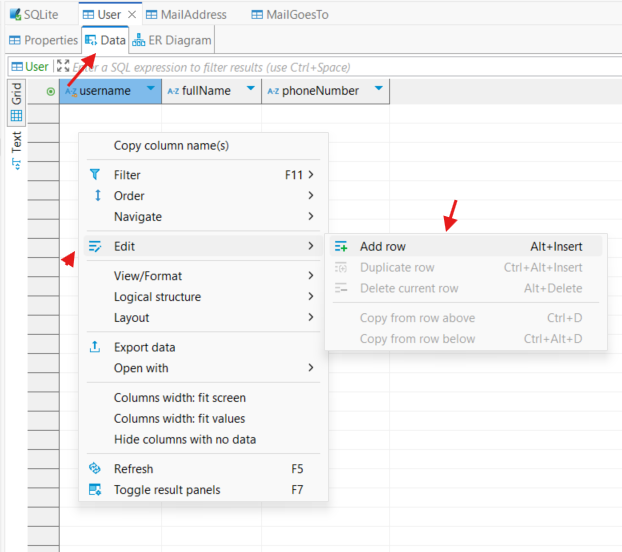
\includegraphics[width=0.7\textwidth]{dbeaver/insert_data_user.png}
  \caption{Insert Data into User in DBeaver.}
  \label{fig:insert_data_user}
\end{figure}

\begin{figure}[!htb]
  \centering
  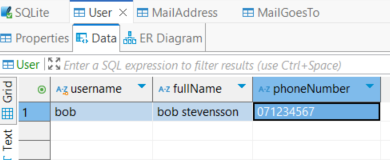
\includegraphics[width=0.7\textwidth]{dbeaver/insert_data_user_populated.png}
  \caption{Bob User Populated in DBeaver.}
  \label{fig:insert_data_user_populated}
\end{figure}


\subsection{Querying Data}
\label{dbeaverQueryingData}

Queries can be written and executed using the views section in DBeaver. The following query will return all columns from the User table where the users full name is ``bob stevensson''.

\begin{lstlisting}[caption={Querying Data in DBeaver}]
SELECT
  *
FROM
  User,
  MailAddress
WHERE
  User.username = MailAddress.createdBy
  AND User.fullName = 'bob stevensson';
\end{lstlisting}

And the process for doing this in DBeaver is as follows:
\begin{enumerate}
  \item Right-click on ``Views'' and choose ``Create New View''. (\autoref{fig:create_view})
  \item Give the view a name and navigate to definition and write the query. (\autoref{fig:view_bob_emails_define})
  \item Press ``Ctrl + S'' (or your operating system's equivalent) to save the view.
  \item Navigate to the ``Data'' tab of the view to see the result. (\autoref{fig:view_bob_emails_result})
\end{enumerate}


\begin{figure}[!htb]
  \centering
  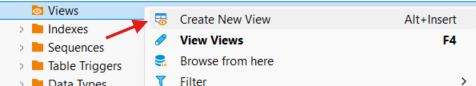
\includegraphics[width=0.7\textwidth]{dbeaver/create_view.png}
  \caption{Create View in DBeaver.}
  \label{fig:create_view}
\end{figure}

\begin{figure}[!htb]
  \centering
  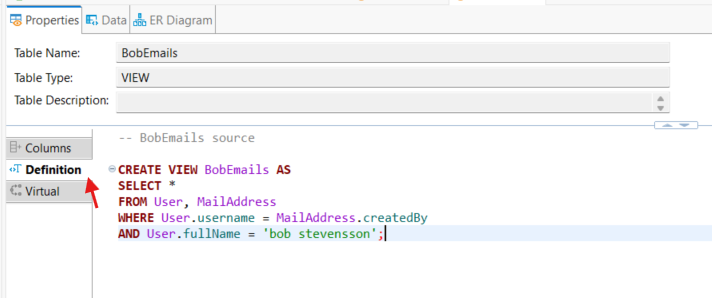
\includegraphics[width=0.7\textwidth]{dbeaver/view_bob_emails_define.png}
  \caption{Define View in DBeaver.}
  \label{fig:view_bob_emails_define}
\end{figure}

\begin{figure}[!htb]
  \centering
  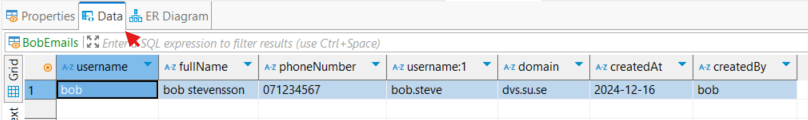
\includegraphics[width=0.8\textwidth]{dbeaver/view_bob_emails_result.png}
  \caption{Result of View in DBeaver.}
  \label{fig:view_bob_emails_result}
\end{figure}

\section{SQLiteStudio}
\label{sqliteStudio}

\subsection{Relevant Known Issues}
\label{sqliteStudioKnownIssues}

\subsubsection{Creating self-referencing foreign keys}
\label{sqliteStudioSelfReferencingForeignKeys}
To create a self-referencing foreign key in SQLiteStudio, for example, a foreign key in the User table that references the User table itself, you will have to create the table without the foreign key first. After that, you can go to the table and add the foreign key.

If the table structure is not properly created/committed before attempting to add the foreign key the target table will not be available in the dropdown list of tables to reference. See \autoref{fig:fnTableNotCommitted} for an example of this.

\begin{figure}[!htb]
  \centering
  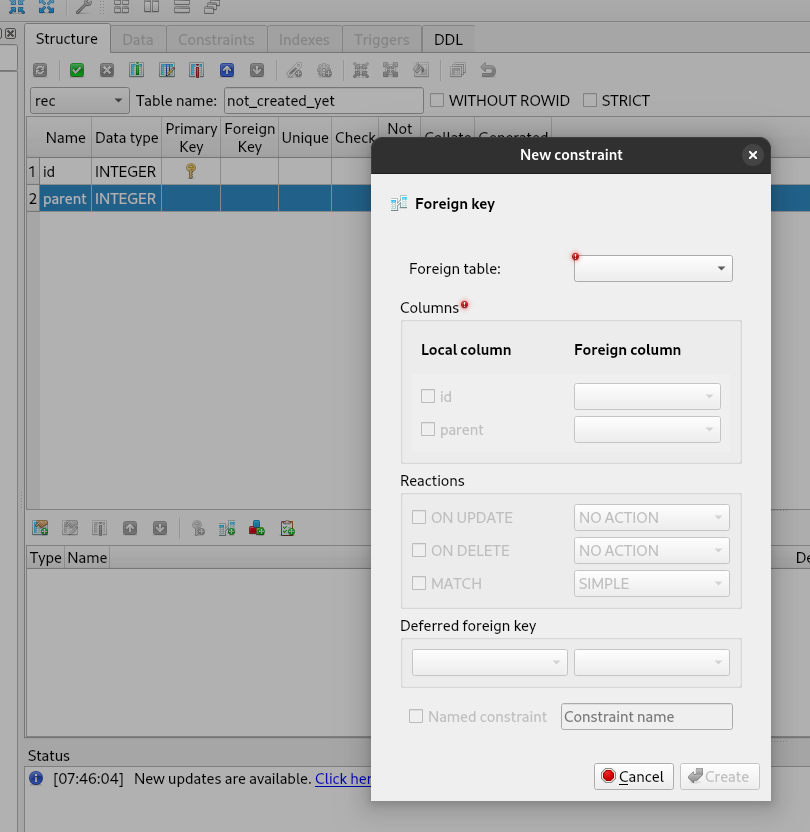
\includegraphics[width=0.8\textwidth]{sqlitestudio/fn_table_not_committed.png}
  \caption{The table is not available in the dropdown list of tables to reference.}
  \label{fig:fnTableNotCommitted}
\end{figure}


\subsection{Common Problems}
\label{sqliteStudioCommonProblems}

\subsubsection{Table Missing}
\label{sqliteStudioTableDisapered}
SQLiteStudio has each table in its own tab, if you accidentally go to a new table and your old one disappeared from your current view. Check the tabs at the bottom of the screen.
\begin{figure}[!htb]
  \centering
  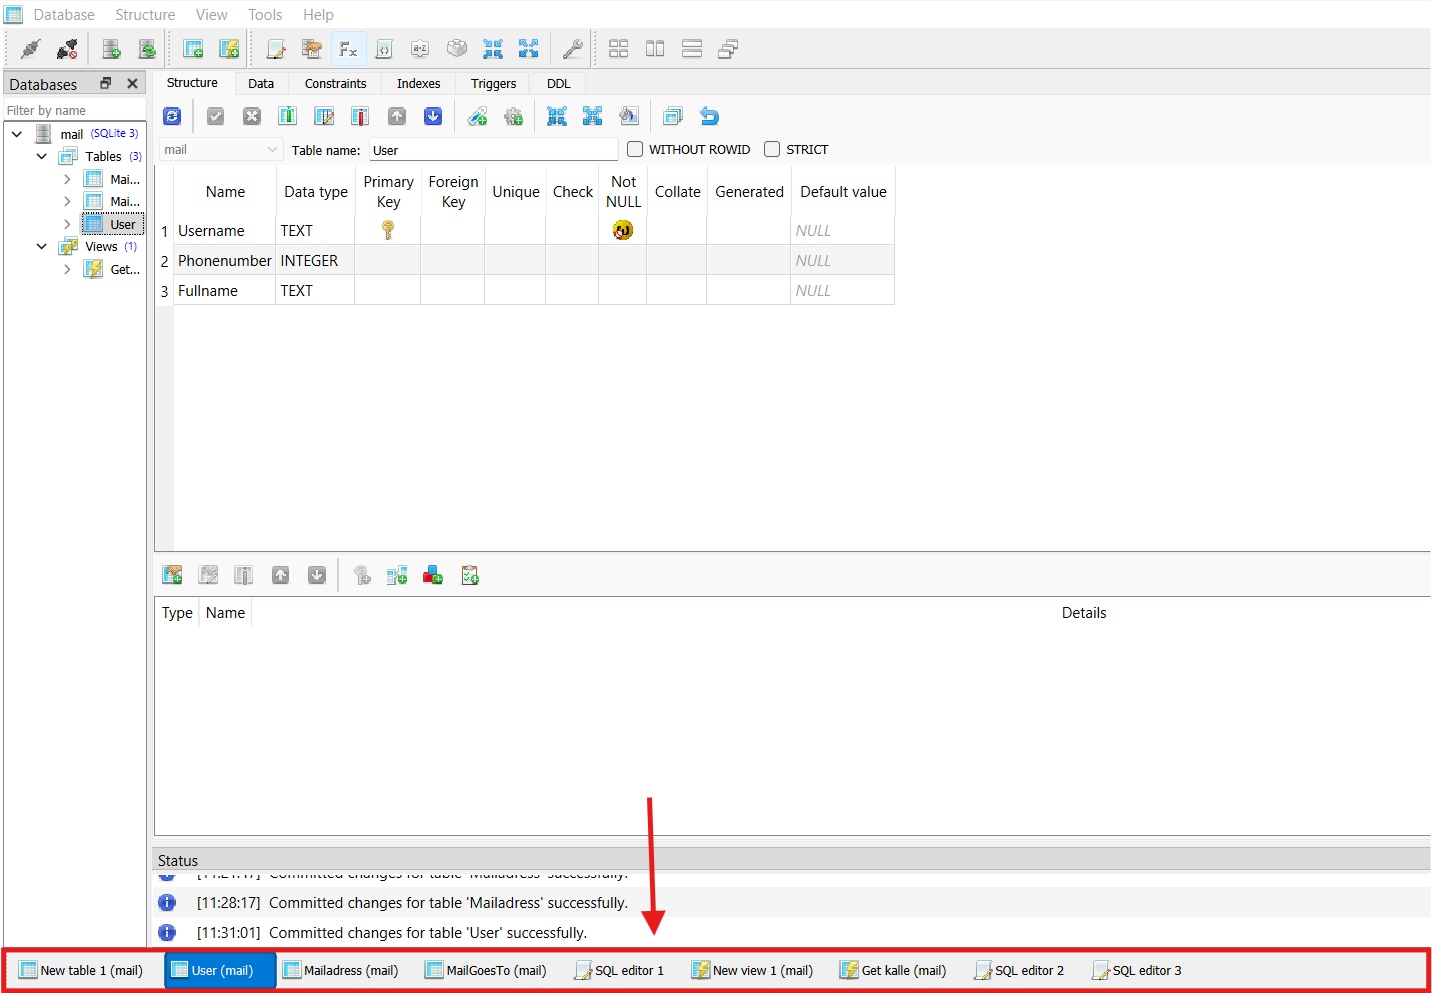
\includegraphics[width=0.7\textwidth]{sqlitestudio/common_problems/table_disapered.png}
  \caption{Table in different window in SQLiteStudio.}
  \label{fig:tabledisapered}
\end{figure}


\subsubsection{No Primary Key}
\label{sqliteStudioNoPrimaryKey}
While creating a table in SQLiteStudio it is possible to create a table without explicitly defining a primary key (this is due to how SQLite handles primary keys). This is not an error, but all tables should have an explicit primary key defined.


% warning wrong datatype on FN (this is a logical error!)
\subsubsection{Wrong Datatype for Foreign Key}
\label{sqliteStudioWrongDatatypeForeignKey}
When creating a foreign key in SQLiteStudio where the datatype of the foreign key column is not the same as the column in the referenced table the program will display a warning. This is usually a logical error and should not be ignored and the datatype in the from or to column should be changed to match. The warning can be seen in \autoref{fig:badfndatatype}.


\begin{figure}[!htb]
  \centering
  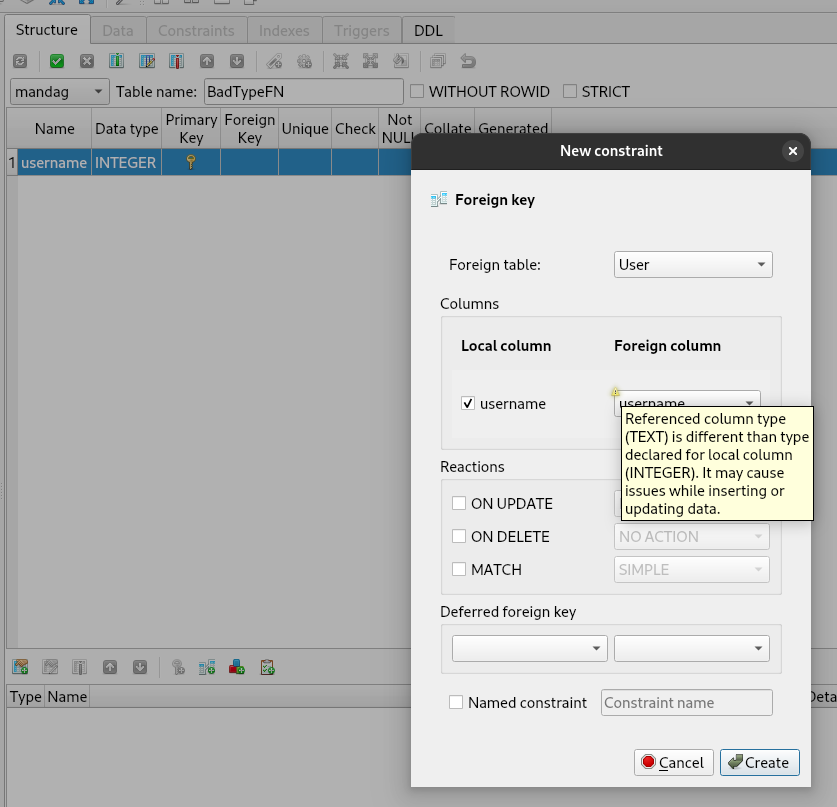
\includegraphics[width=0.8\textwidth]{sqlitestudio/badfndatatype.png}
  \caption{Wrong Datatype for Foreign Key Column in SQLiteStudio.}
  \label{fig:badfndatatype}
\end{figure}




% \subsection{Implementation of the Database Model}
% \label{sqliteStudioImplementation}

\subsection{Creating a Database}
\label{sqliteStudioCreatingDatabase}
To create a database in SQLiteStudio start by pressing the button Database in the top left corner. After that you will get a popup \autoref{fig:createDBpopupblank}
\begin{figure}[!htb]
  \centering
  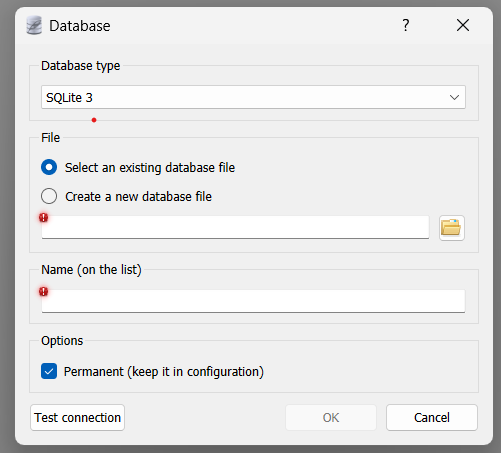
\includegraphics[width=0.7\textwidth]{sqlitestudio/create_database/create_database_popup.png}
  \caption{Popup for creating a new database in SQLiteStudio.}
  \label{fig:createDBpopupblank}
\end{figure}
Select create a new database. The text field under the path to where you want to store your database, click on the folder next to it and navigate to the folder you want to store your database in. I suggest creating a folder in documents to store the database in. After selecting your folder you should enter the filename following this format ``Example.db3'', as you can see in \autoref{fig:createDBnavigate} I called it mail.db  
\begin{figure}[!htb]
  \centering
  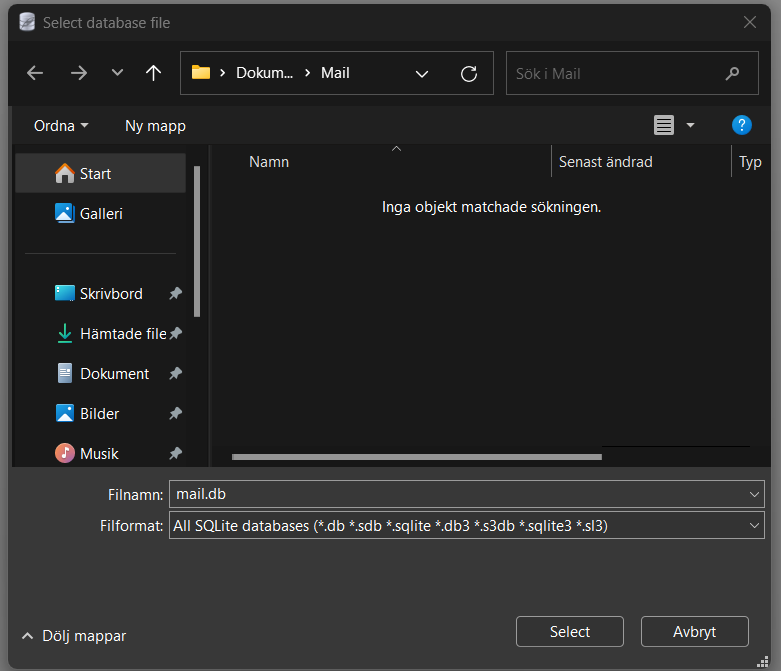
\includegraphics[width=0.7\textwidth]{sqlitestudio/create_database/create_database_navigate.png}
  \caption{Example for how to select the folder you want to store your database in.}
  \label{fig:createDBnavigate}
\end{figure}
The name text field is where you enter the name of your database. \autoref{fig:createDBfilled}
\begin{figure}[!htb]
  \centering
  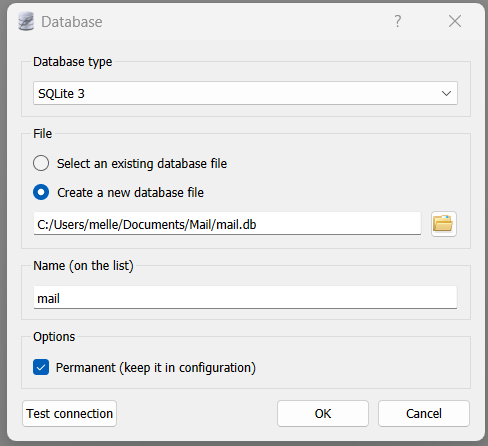
\includegraphics[width=0.7\textwidth]{sqlitestudio/create_database/create_database_populated.png}
  \caption{How the popup should look when entered everything.}
  \label{fig:createDBfilled}
\end{figure}
After that you can press OK, and your database will be created. The database will appear in left under ``Databases''.

\subsection{Creating a Table}
\label{sqliteStudioCreatingTable}
To create a table in SQLiteStudio star by clicking in your database to get tables and views. Then right-click on the tables and selected create new table. \autoref{fig:createTableRightClick}

\begin{figure}[!htb]
  \centering
  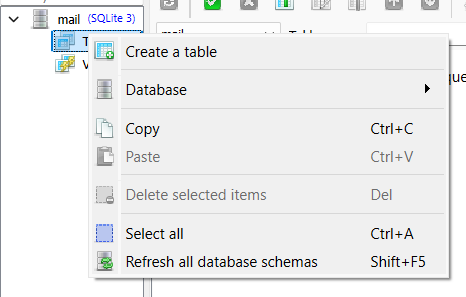
\includegraphics[width=0.7\textwidth]{sqlitestudio/create_table/create_table_right_clicked.png}
  \caption{The dropout menu for creating a new table in SQLiteStudio.}
  \label{fig:createTableRightClick}
\end{figure}
In this section we will create the User table and the MailAddress table. The rest of the tables can be created similarly, and are as such left as an exercise for the reader. We will only cover the creation of the primary keys of User and MailAddress Tables because the rest of the columns are created similarly, with the difference that you don't mark them as primary keys.


\subsubsection{User Table}
\label{sqliteStudioUserTable}
After selecting create new table you will be presented with a blank table, see \autoref{fig:CreateTableBlanktable} you start by entering the name, this is going to be the user table.
\begin{figure}[!htb]
  \centering
  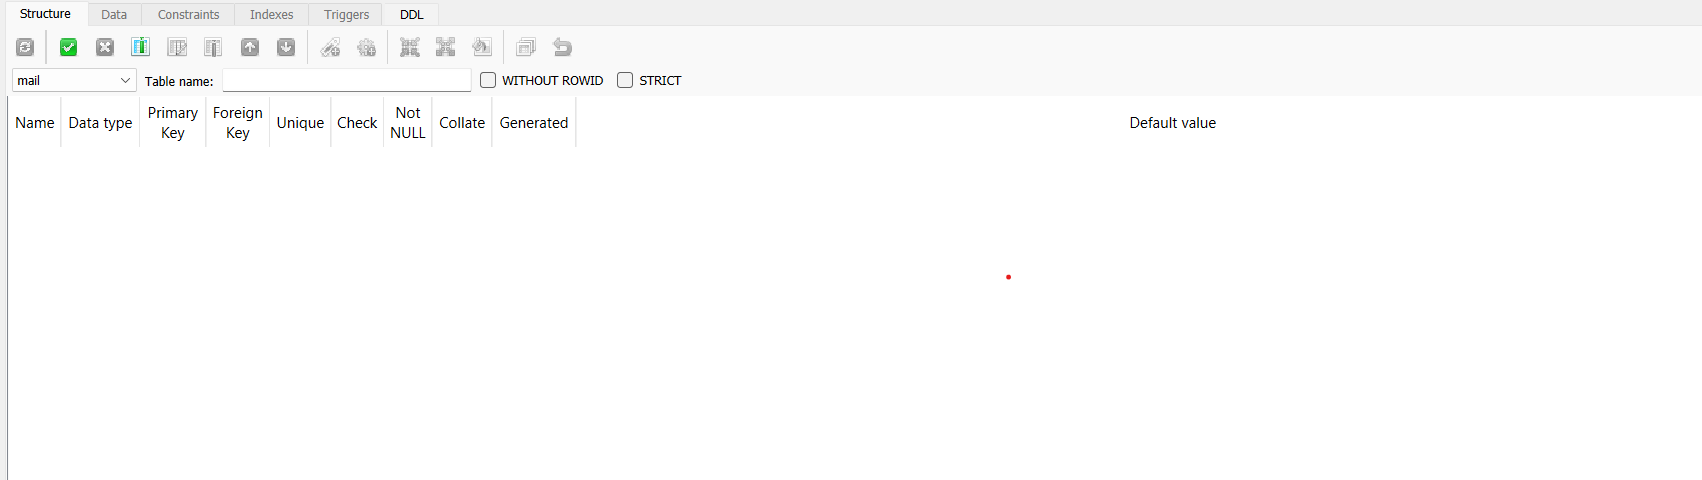
\includegraphics[width=0.7\textwidth]{sqlitestudio/create_table/create_table_blank.png}
  \caption{The dropout menu for creating a new table in SQLiteStudio.}
  \label{fig:CreateTableBlanktable}
\end{figure}
At the top of the user table all options will be greyed out except for ``commit structure changes'' and ``add column''. Press add column. You will be presented with the window to create a column, \autoref{fig:BlankNewColumn}. 
\begin{figure}[!htb]
  \centering
  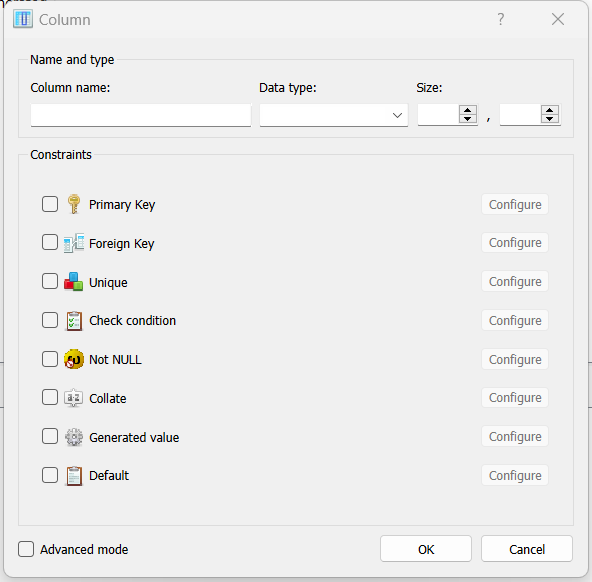
\includegraphics[width=0.7\textwidth]{sqlitestudio/create_table/create_table_column_blank.png}
  \caption{Blank menu for creating a new column in SQLiteStudio.}
  \label{fig:BlankNewColumn}
\end{figure}
The first column we will create is the username column. The name of the column is username and then select the datatype from the list next to the name of the column. We will make it the primary key and set it to NOT NULL by checking the boxes, \autoref{fig:FilledNewColumnUser}. 
\begin{figure}[!htb]
  \centering
  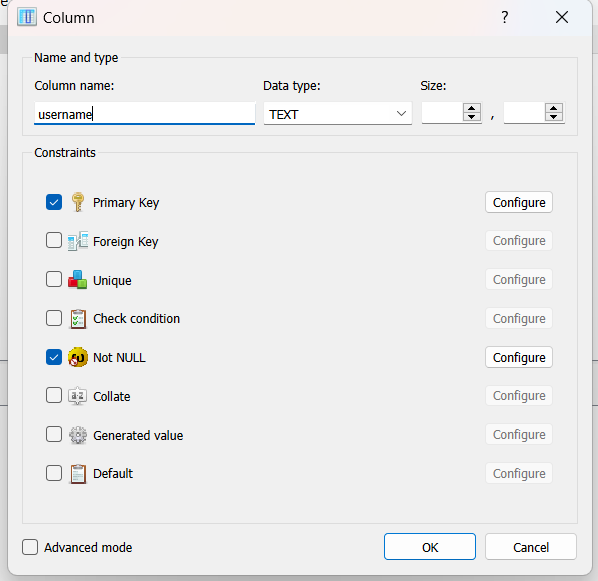
\includegraphics[width=0.7\textwidth]{sqlitestudio/create_user/create_user_column_populated.png}
  \caption{Filled menu for creating a new column in SQLiteStudio.}
  \label{fig:FilledNewColumnUser}
\end{figure}
Now you can press ``Commit structure changes'' to save the table. Then you will get a window with a SQL query that will be executed to create the table, you don't need to do anything here just press OK. 

You can repeat the steps from adding the username column to add the fullName and phoneNumber columns.   

\subsubsection{MailAddress Table}
\label{sqliteStudioMailAddressTable}
MailAddress table is created in the same way as the User table. The only difference is that the primary key is a composite key. It is both the username and domain columns. We will start with the same steps and creating a new table as we did with the User table. After that we will add the username and domain columns, checking both as NOT NULL but importantly not as a primary key! The table should look like \autoref{fig:MailAddressTableNoKeys}.
\begin{figure}[!htb]
  \centering
  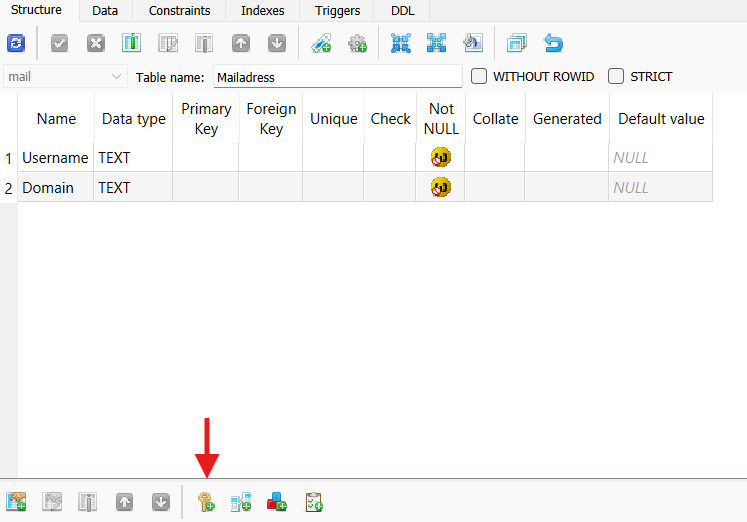
\includegraphics[width=0.7\textwidth]{sqlitestudio/create_mail_address/create_mail.png}
  \caption{Created two columns in MailAddress table which are not primary keys.} 
  \label{fig:MailAddressTableNoKeys}
\end{figure}

In the items on the bottom of the table view you can see a key icon, press this button, \autoref{fig:MailAddressTablePrimaryKeys}. You will be presented with a window where you can select the columns that should be part of the primary key, \autoref{fig:MailAddressTablePrimaryKeys}. 
\begin{figure}[!htb]
  \centering
  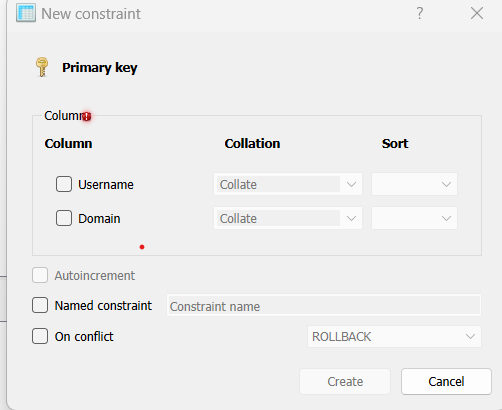
\includegraphics[width=0.7\textwidth]{sqlitestudio/create_mail_address/create_mail_blank_primary_keys.png}
  \caption{Menu for adding primary keys in MailAddress table.}
  \label{fig:MailAddressTablePrimaryKeys}
\end{figure}
Select the username and domain columns. You can and should (for now) ignore the rest of the options in the window. Press create and then press ``Commit structure changes'' to save the table. After that you can create the rest of the columns in the same way as you did with the User table. If you got a key eye for UML diagrams you can see that username will be a foreign key in MailAddress table, foreign keys will be covered later under the chapter Foreign Keys.  
\subsubsection{MailGoesTo Table}
\label{sqliteStudioMailGoesToTable}
MailGoesTo is table created to handle a many-to-many relationship between inbox and MailAddress tables. This means both of it keys will be foreign keys to other tables. You don't have to worry about foreign keys as they will be covered in more detail later. As the rules on creating a table for a many-to-many relationship the primary keys in MailGoesTo will the primary keys of Inbox and MailAddress. Nothing new will be covered in this section, as such this will be left as an exercise. After creating the table it should look like \autoref{fig:MailGoesToTable}. 
\begin{figure}[!htb]
  \centering
  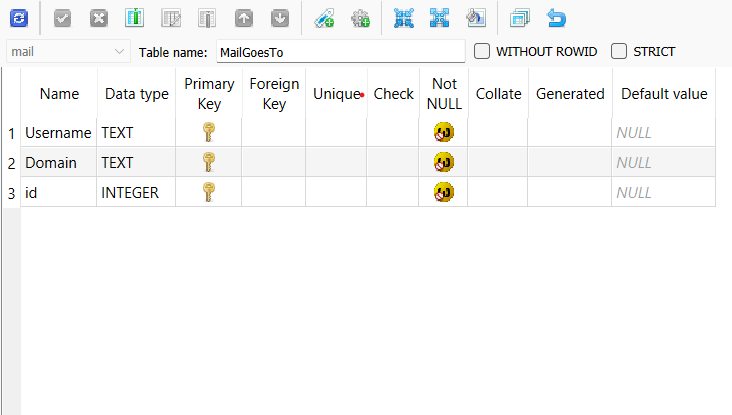
\includegraphics[width=0.7\textwidth]{sqlitestudio/create_mail_goes_to/create_mail_goes_to.png}
  \caption{Completed MailGoesTo table.}
  \label{fig:MailGoesToTable}
\end{figure}
\subsection{Alternative Keys}
\label{sqliteStudioAlternativeKeys}
To create an alternative key in SQLiteStudio you press the button with three colored squares, \autoref{fig:FindUniqueButton}. 
\begin{figure}[!htb]
  \centering
  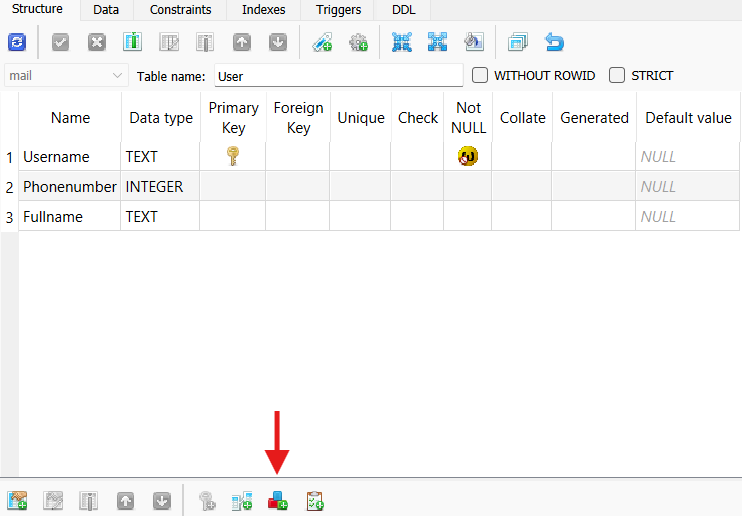
\includegraphics[width=0.7\textwidth]{sqlitestudio/alternative_key/unique_symbol_square.png}
  \caption{Finding the unique button in SQLiteStudio.}
  \label{fig:FindUniqueButton}
\end{figure}
After which you will be presented with a window where you can select the columns that should be part of the alternative key, \autoref{fig:UniqueBlankWindow}.
\begin{figure}[!htb]
  \centering
  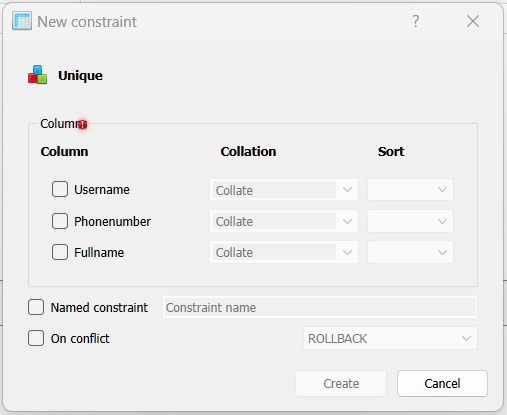
\includegraphics[width=0.7\textwidth]{sqlitestudio/alternative_key/alternative_key_blank.png}
  \caption{Unique window in SQLiteStudio.}
  \label{fig:UniqueBlankWindow}
\end{figure}
To demonstrate we will create a composite key of the columns fullName and phoneNumber in the User table. After selecting the columns you can press the key icon to create the key. You can see that the alternative is created in the area below the table view, \autoref{fig:SucessAlternativeKey}.
\begin{figure}[!htb]
  \centering
  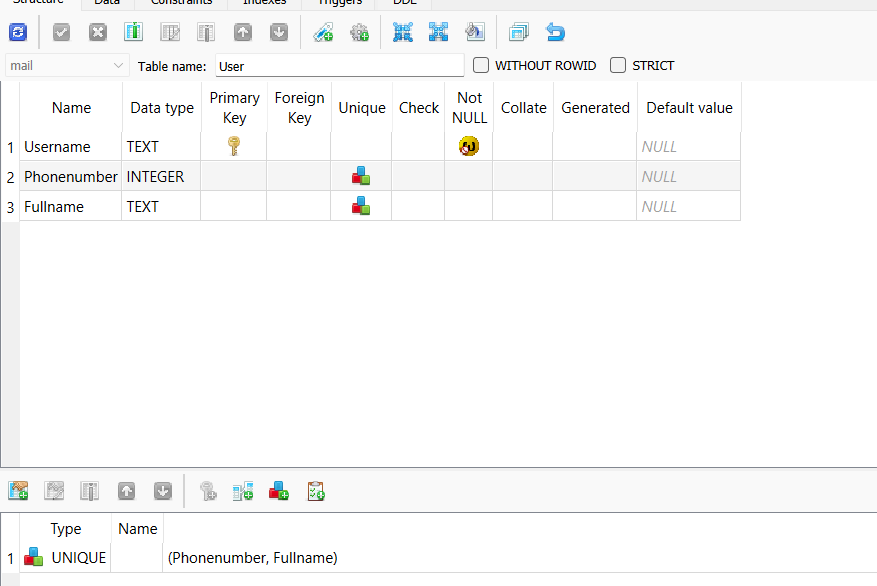
\includegraphics[width=0.7\textwidth]{sqlitestudio/alternative_key/alternative_key_success.png}
  \caption{Table view for user table with the alternative key.}
  \label{fig:SucessAlternativeKey}
\end{figure}

\subsection{Foreign Keys}
\label{sqliteStudioForeignKeys}
In between the primary key icon and three squares there is a picture of two tables with a link between them, press this button, \autoref{fig:MailAddressForeignKeysButton}.
\begin{figure}[!htb]
  \centering
  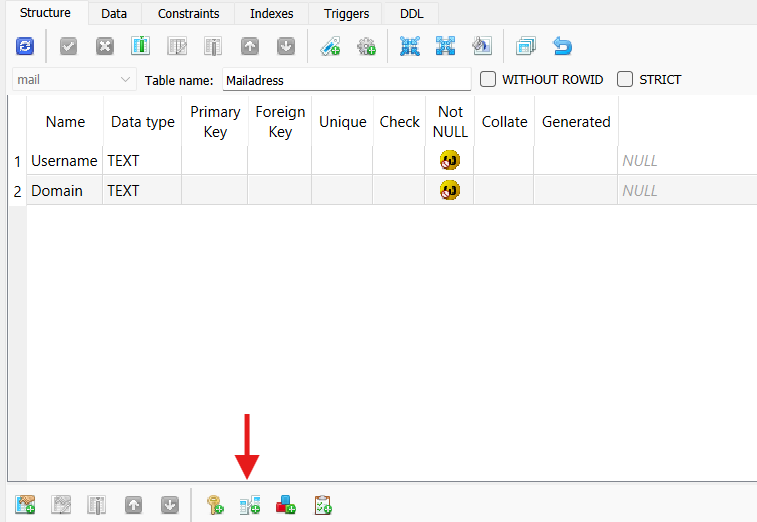
\includegraphics[width=0.7\textwidth]{sqlitestudio/create_foreign_key/foreign_key_button_location.png}
  \caption{View over MailAddress table with the button for creating a foreign key.}
  \label{fig:MailAddressForeignKeysButton}
\end{figure}
The window (\autoref{fig:MailAddressForeignKeysBlankWindow}) will allow you to select a foreign table and the columns that should be part of the foreign key.
\begin{figure}[!htb]
  \centering
  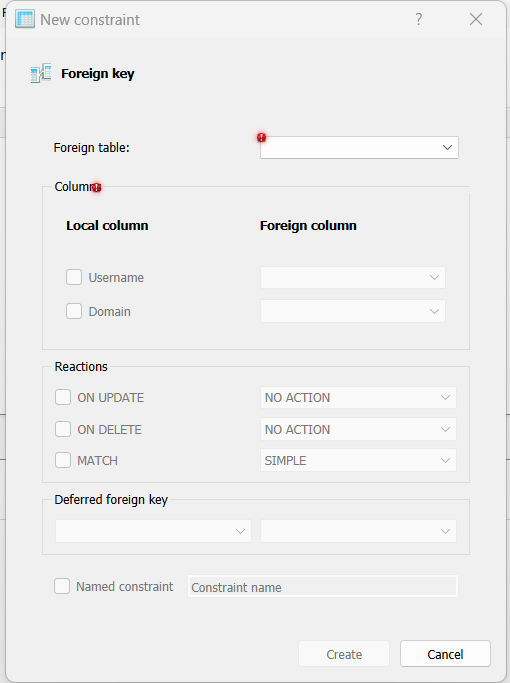
\includegraphics[width=0.7\textwidth]{sqlitestudio/create_foreign_key/foreign_key_blank.png}
  \caption{Popup to create a foreign key}
  \label{fig:MailAddressForeignKeysBlankWindow}
\end{figure}
We will create a foreign key between the username column in MailAddress and the username column in User. After selecting you local column you can enter what it corresponds to by selecting it in the drop-down list across, \autoref{fig:MailAddressForeignKeysDropDown}. 
\begin{figure}[!htb]
  \centering
  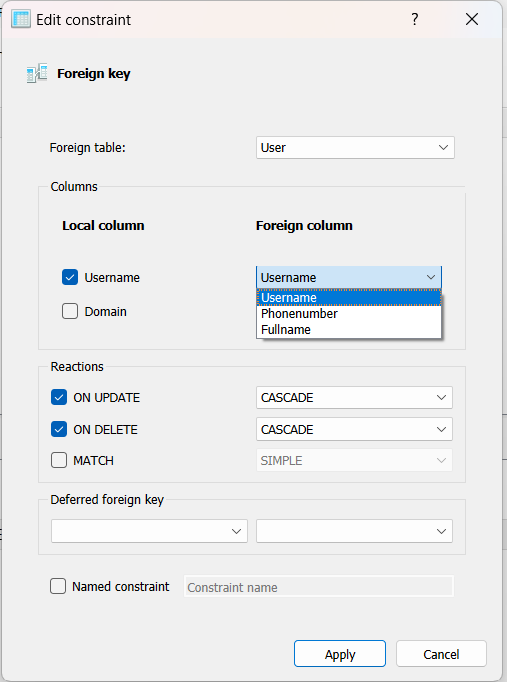
\includegraphics[width=0.7\textwidth]{sqlitestudio/create_foreign_key/foreign_key_dropdown_menu.png}
  \caption{Popup to create a foreign key}
  \label{fig:MailAddressForeignKeysDropDown}
\end{figure}
You can also set condition for if the key it referencing is deleted or updated, for example, a person changes their username. Set the behavior to what is appropriate for your case, see \autoref{fig:MailAddressForeignKeysFilledWindow}. Then press create, and the foreign key will be created.
\begin{figure}[!htb]
  \centering
  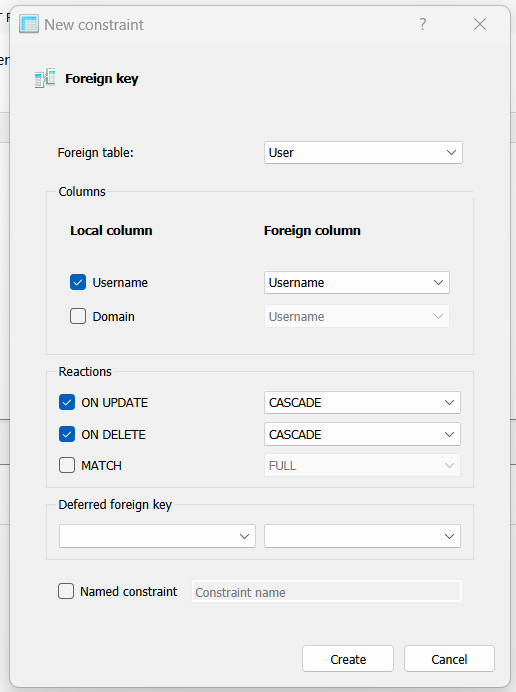
\includegraphics[width=0.7\textwidth]{sqlitestudio/create_foreign_key/foreign_key_populated.png}
  \caption{Filled popup to create foreign key}
  \label{fig:MailAddressForeignKeysFilledWindow}
\end{figure}   
In MailGoesTo we have two columns that are part of the same foreign key and have to create a composite key with both columns. Follow the same steps as previously with the difference that you select both columns instead of just one, see \autoref{fig:MailAddressForeignKeysComposit}. After that press create and the foreign key will be created.
\begin{figure}[!htb]
  \centering
  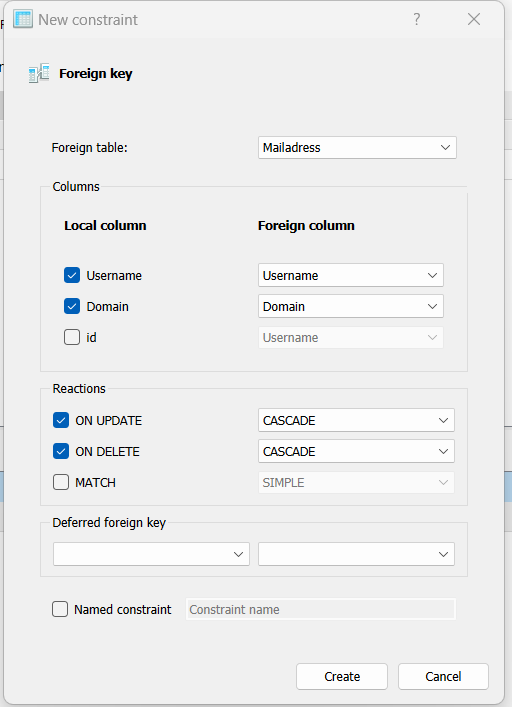
\includegraphics[width=0.7\textwidth]{sqlitestudio/create_foreign_key/composite_foreign_key.png}
  \caption{Filled popup to create composite foreign key}
  \label{fig:MailAddressForeignKeysComposit}
\end{figure}   
\subsection{Inserting Data}
\label{sqliteStudioInsertingData}
To insert data in SQLiteStudio you press the data button, \autoref{fig:insertdataFindDataView}, on the top of table view. 
\begin{figure}[!htb]
  \centering
  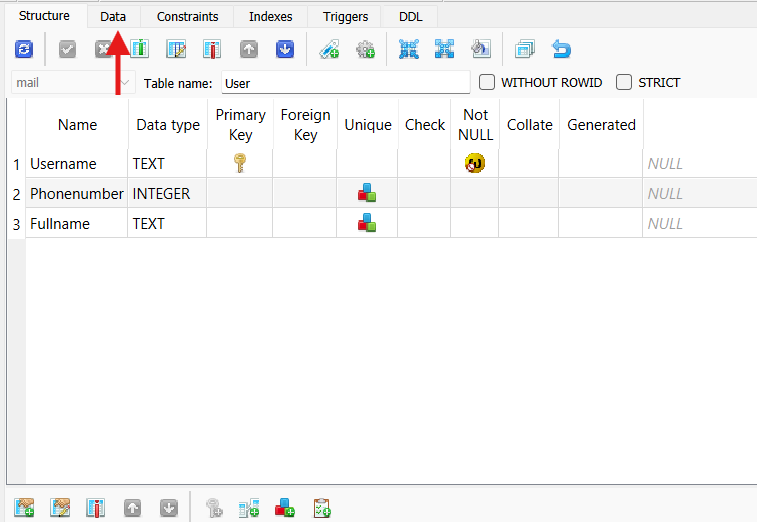
\includegraphics[width=0.7\textwidth]{sqlitestudio/insert_data/insert_data_find_view.png}
  \caption{Table view for user table}
  \label{fig:insertdataFindDataView}
\end{figure}
After pressing it you will be presented with a data window, see \autoref{fig:insertdataDataViewBlank}.
\begin{figure}[!htb]
  \centering
  \includegraphics[width=0.7\textwidth]{sqlitestudio/insert_data/insert_data_view_blank.png}
  \caption{Data view for user table}
  \label{fig:insertdataDataViewBlank}
\end{figure}
Press the green plus to add a row. You can now enter the data for the columns in the table.
%Exists image with blank row was demend to not be needed
\begin{figure}[!htb]
  \centering
  \includegraphics[width=0.7\textwidth]{sqlitestudio/insert_data/insert_data_row_populated.png}
  \caption{Data view with data}
  \label{fig:InsertdataROWFILLED}
\end{figure}
Press the green checkmark to save the data, \autoref{fig:InsertdataROWFILLED}. 
  
\subsection{Querying Data}
\label{sqliteStudioQueryingData}
To create and run a query, can be done by either pressing create view or open SQL editor, see \autoref{fig:Findquery}.
\begin{figure}[!htb]
  \centering
  \includegraphics[width=0.7\textwidth]{sqlitestudio/queries/create_query_find.png}
  \caption{Find query buttons}
  \label{fig:Findquery}
\end{figure} 
Using CREATE VIEW may be beneficial as it will save your queries. After pressing create view you will be presented with a blank window (\autoref{fig:blankquery}) where you can write your query and in the top you can enter your view name.
\begin{figure}[!htb]
  \centering
  \includegraphics[width=0.7\textwidth]{sqlitestudio/queries/create_query_blank.png}
  \caption{Blank new view}
  \label{fig:blankquery}
\end{figure} 
After you have written your query you can press the green checkmark to save the view. 

To see the result you need to enter into data view, see \autoref{fig:Resultsquery}.
\begin{figure}[!htb]
  \centering
  \includegraphics[width=0.7\textwidth]{sqlitestudio/queries/create_query_find_results.png}
  \caption{Results from the query} 
  \label{fig:Resultsquery}
\end{figure} 
All saved views will be shown in the view list right below your tables, \autoref{fig:Allviews}.  
\begin{figure}[!htb]
  \centering
  \includegraphics[width=0.7\textwidth]{sqlitestudio/queries/create_query_find_views.png}
  \caption{All views in the database} 
  \label{fig:Allviews}
\end{figure} 

\section{SQLite ERD}
\label{sqliteERD}
SQLite ERD is an application that can be used to create Entity Relationship Diagrams (ERDs) for SQLite databases. The application is platform-independent and is used within a web browser. The application can be found at \url{https://sqlite-erd.e-su.se/}. For the interested reader, the source code can be found at \url{https://github.com/Edwinexd/sqlite-erd}.
The application supports most common file formats for SQLite databases, only requiring that the file is a SQLite database of version 3.

The application also performs some semantic analysis on the database, such as checking for foreign key datatypes and ensuring that foreign columns are unique.

The complete implemented database model can be seen in, \autoref{fig:modelSQLiteERD}

\begin{figure}[!htb]
  \centering
  \includegraphics[width=1\textwidth]{model/sqlite_erd.png}
  \caption{The table is not available in the dropdown list of tables to reference.}
  \label{fig:modelSQLiteERD}
\end{figure}

\section{Final Words}
\label{finalWords}
If you have any questions or issues with the tools presented in this document or the document itself, please create an issue at \url{https://github.com/Edwinexd/db-sqlite-tools/issues}.

\pagebreak
\bibliographystyle{IEEEtran}
\bibliography{bibtex}
\bibdata{bibtex}

\end{sloppypar}
\end{document}
